\documentclass{standalone}
\usepackage{tikz}
\usetikzlibrary{patterns, positioning}
\usepackage[sfdefault]{ClearSans} %% option 'sfdefault' activates Clear Sans as the default text font
\usepackage[T1]{fontenc}

\begin{document}
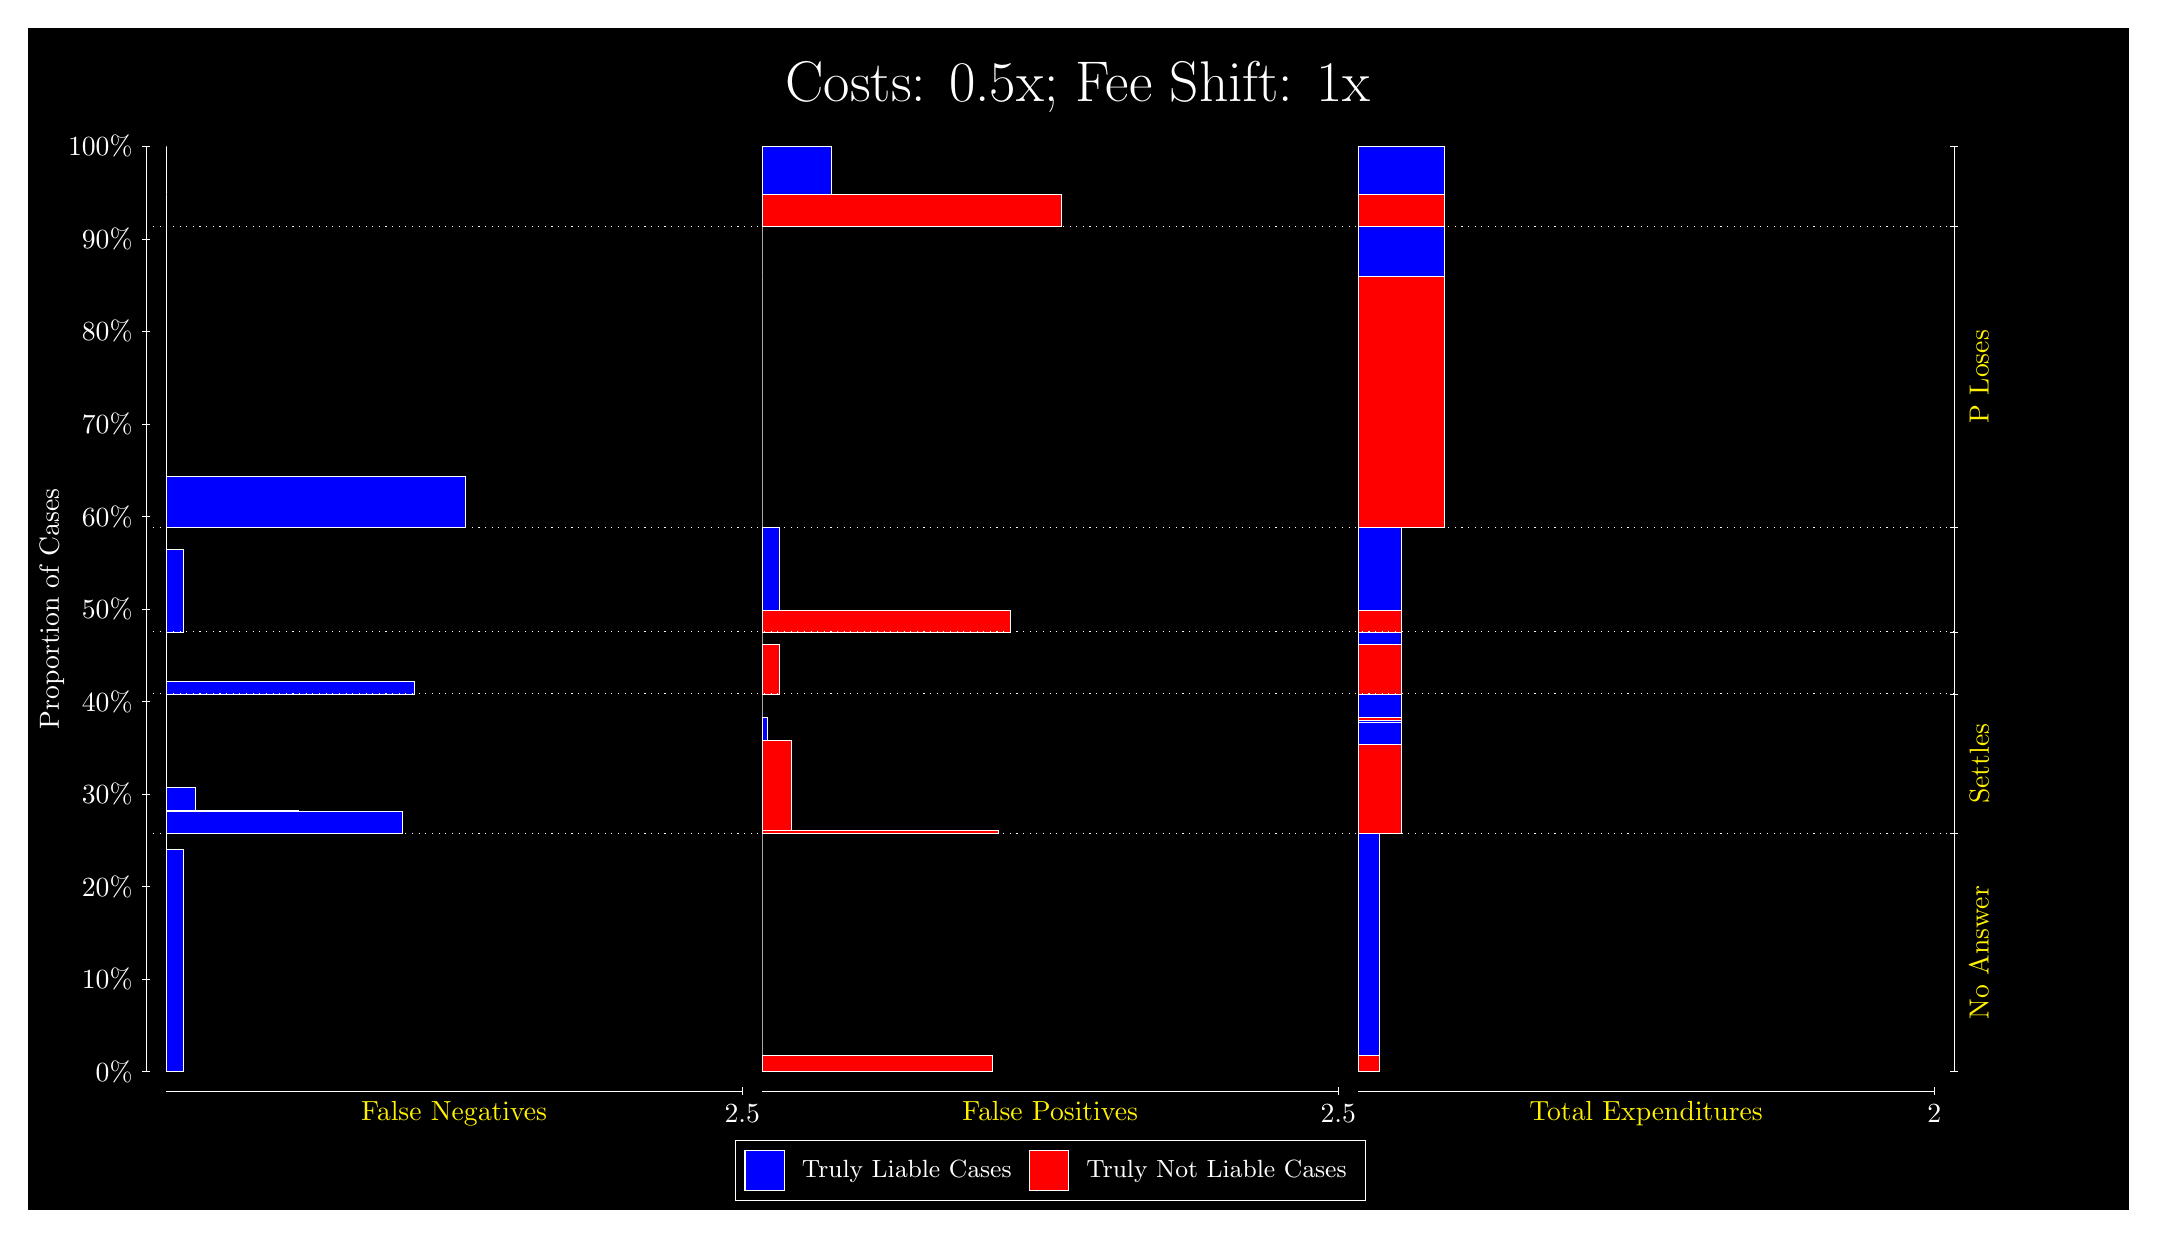
\begin{tikzpicture}
\draw[fill=black] (0,0) rectangle (26.667,15);
\draw[text=white] (0,13.5) rectangle (26.667,15) node[midway] {\huge Costs: 0.5x; Fee Shift: 1x};
\draw[white, very thin] (1.5,1.75) -- (1.5,13.5);
\node[rotate=90, text=white, anchor=center] at (0.3, 7.625) {Proportion of Cases};
\draw[white, very thin] (1.45,1.75) -- (1.55,1.75);
\node[text=white, anchor=east] at (1.45, 1.75) {0\%};
\draw[white, very thin] (1.45,2.925) -- (1.55,2.925);
\node[text=white, anchor=east] at (1.45, 2.925) {10\%};
\draw[white, very thin] (1.45,4.1) -- (1.55,4.1);
\node[text=white, anchor=east] at (1.45, 4.1) {20\%};
\draw[white, very thin] (1.45,5.275) -- (1.55,5.275);
\node[text=white, anchor=east] at (1.45, 5.275) {30\%};
\draw[white, very thin] (1.45,6.45) -- (1.55,6.45);
\node[text=white, anchor=east] at (1.45, 6.45) {40\%};
\draw[white, very thin] (1.45,7.625) -- (1.55,7.625);
\node[text=white, anchor=east] at (1.45, 7.625) {50\%};
\draw[white, very thin] (1.45,8.8) -- (1.55,8.8);
\node[text=white, anchor=east] at (1.45, 8.8) {60\%};
\draw[white, very thin] (1.45,9.975) -- (1.55,9.975);
\node[text=white, anchor=east] at (1.45, 9.975) {70\%};
\draw[white, very thin] (1.45,11.15) -- (1.55,11.15);
\node[text=white, anchor=east] at (1.45, 11.15) {80\%};
\draw[white, very thin] (1.45,12.325) -- (1.55,12.325);
\node[text=white, anchor=east] at (1.45, 12.325) {90\%};
\draw[white, very thin] (1.45,13.5) -- (1.55,13.5);
\node[text=white, anchor=east] at (1.45, 13.5) {100\%};

\draw[white, very thin] (24.457,1.75) -- (24.457,13.5);
\draw[white, very thin] (24.407,1.75) -- (24.507,1.75);
\node[anchor=west] at (24.407, 1.75) {};
\draw[white, very thin] (24.407,4.7727) -- (24.507,4.7727);
\node[anchor=west] at (24.407, 4.7727) {};
\draw[white, very thin] (24.407,6.5457) -- (24.507,6.5457);
\node[anchor=west] at (24.407, 6.5457) {};
\draw[white, very thin] (24.407,7.3347) -- (24.507,7.3347);
\node[anchor=west] at (24.407, 7.3347) {};
\draw[white, very thin] (24.407,8.6645) -- (24.507,8.6645);
\node[anchor=west] at (24.407, 8.6645) {};
\draw[white, very thin] (24.407,12.487) -- (24.507,12.487);
\node[anchor=west] at (24.407, 12.487) {};
\draw[white, very thin] (24.407,13.5) -- (24.507,13.5);
\node[anchor=west] at (24.407, 13.5) {};

\draw[white, very thin, fill=blue] (1.75,1.75) rectangle (1.9696,4.5692);
\draw[white, very thin, fill=red] (1.75,4.5692) rectangle (1.75,4.7727);
\draw[white, very thin, fill=blue] (1.75,4.7727) rectangle (4.7507,5.0538);
\draw[white, very thin, fill=blue] (1.75,5.0538) rectangle (3.4333,5.0704);
\draw[white, very thin, fill=blue] (1.75,5.0704) rectangle (2.1159,5.3644);
\draw[white, very thin, fill=red] (1.75,5.3644) rectangle (1.75,6.5457);
\draw[white, very thin, fill=blue] (1.75,6.5457) rectangle (4.8971,6.7071);
\draw[white, very thin, fill=red] (1.75,6.7071) rectangle (1.75,7.3347);
\draw[white, very thin, fill=blue] (1.75,7.3347) rectangle (1.9696,8.3852);
\draw[white, very thin, fill=red] (1.75,8.3852) rectangle (1.75,8.6645);
\draw[white, very thin, fill=blue] (1.75,8.6645) rectangle (5.5558,9.3072);
\draw[white, very thin, fill=red] (1.75,9.3072) rectangle (1.75,12.487);
\draw[white, very thin, fill=red] (1.75,12.487) rectangle (1.75,12.891);
\draw[white, very thin, fill=blue] (1.75,12.891) rectangle (1.75,13.5);
\draw[white, very thin, fill=red] (9.3189,1.75) rectangle (12.246,1.9535);
\draw[white, very thin, fill=blue] (9.3189,1.9535) rectangle (9.3189,4.7727);
\draw[white, very thin, fill=red] (9.3189,4.7727) rectangle (12.32,4.8161);
\draw[white, very thin, fill=red] (9.3189,4.8161) rectangle (11.002,4.8193);
\draw[white, very thin, fill=red] (9.3189,4.8193) rectangle (9.6848,5.954);
\draw[white, very thin, fill=blue] (9.3189,5.954) rectangle (9.3921,6.248);
\draw[white, very thin, fill=blue] (9.3189,6.248) rectangle (9.3189,6.5457);
\draw[white, very thin, fill=red] (9.3189,6.5457) rectangle (9.5384,7.1733);
\draw[white, very thin, fill=blue] (9.3189,7.1733) rectangle (9.3189,7.3347);
\draw[white, very thin, fill=red] (9.3189,7.3347) rectangle (12.466,7.6139);
\draw[white, very thin, fill=blue] (9.3189,7.6139) rectangle (9.5384,8.6645);
\draw[white, very thin, fill=red] (9.3189,8.6645) rectangle (9.3189,11.845);
\draw[white, very thin, fill=blue] (9.3189,11.845) rectangle (9.3189,12.487);
\draw[white, very thin, fill=red] (9.3189,12.487) rectangle (13.125,12.891);
\draw[white, very thin, fill=blue] (9.3189,12.891) rectangle (10.197,13.5);
\draw[white, very thin, fill=red] (16.888,1.75) rectangle (17.162,1.9535);
\draw[white, very thin, fill=blue] (16.888,1.9535) rectangle (17.162,4.7727);
\draw[white, very thin, fill=red] (16.888,4.7727) rectangle (17.437,5.9074);
\draw[white, very thin, fill=blue] (16.888,5.9074) rectangle (17.437,6.1885);
\draw[white, very thin, fill=red] (16.888,6.1885) rectangle (17.437,6.1917);
\draw[white, very thin, fill=blue] (16.888,6.1917) rectangle (17.437,6.2083);
\draw[white, very thin, fill=red] (16.888,6.2083) rectangle (17.437,6.2517);
\draw[white, very thin, fill=blue] (16.888,6.2517) rectangle (17.437,6.5457);
\draw[white, very thin, fill=red] (16.888,6.5457) rectangle (17.437,7.1733);
\draw[white, very thin, fill=blue] (16.888,7.1733) rectangle (17.437,7.3347);
\draw[white, very thin, fill=red] (16.888,7.3347) rectangle (17.437,7.6139);
\draw[white, very thin, fill=blue] (16.888,7.6139) rectangle (17.437,8.6645);
\draw[white, very thin, fill=red] (16.888,8.6645) rectangle (17.986,11.845);
\draw[white, very thin, fill=blue] (16.888,11.845) rectangle (17.986,12.487);
\draw[white, very thin, fill=red] (16.888,12.487) rectangle (17.986,12.891);
\draw[white, very thin, fill=blue] (16.888,12.891) rectangle (17.986,13.5);
\draw[white, dotted] (1.5,4.7727) -- (24.457,4.7727);
\draw[white, dotted] (1.5,6.5457) -- (24.457,6.5457);
\draw[white, dotted] (1.5,7.3347) -- (24.457,7.3347);
\draw[white, dotted] (1.5,8.6645) -- (24.457,8.6645);
\draw[white, dotted] (1.5,12.487) -- (24.457,12.487);
\draw[white, very thin] (1.75,1.5) -- (9.0689,1.5);
\node[text=yellow, anchor=north] at (5.4094, 1.5) {False Negatives};
\draw[white, very thin] (9.0689,1.45) -- (9.0689,1.55);
\node[text=white, anchor=north] at (9.0689, 1.45) {2.5};

\draw[white, very thin] (9.3189,1.5) -- (16.638,1.5);
\node[text=yellow, anchor=north] at (12.978, 1.5) {False Positives};
\draw[white, very thin] (16.638,1.45) -- (16.638,1.55);
\node[text=white, anchor=north] at (16.638, 1.45) {2.5};

\draw[white, very thin] (16.888,1.5) -- (24.207,1.5);
\node[text=yellow, anchor=north] at (20.547, 1.5) {Total Expenditures};
\draw[white, very thin] (24.207,1.45) -- (24.207,1.55);
\node[text=white, anchor=north] at (24.207, 1.45) {2};

\node[text=yellow, centered, rotate=90] at (24.777, 3.2614) {No Answer};
\node[text=yellow, centered, rotate=90] at (24.777, 5.6592) {Settles};


\node[text=yellow, centered, rotate=90] at (24.777, 10.576) {P Loses};


\draw (12.978300999999998,1.5) node[draw=none] (baseCoordinate) {};
\begin{scope}[align=center]
        \matrix[scale=0.5, draw=white, below=0.5cm of baseCoordinate, nodes={draw}, column sep=0.1cm]{
            \node[rectangle, draw, minimum width=0.5cm, minimum height=0.5cm, fill=blue] {}; &
            \node[draw=none, font=\small, text=white] (B) {Truly Liable Cases}; &
            \node[rectangle, draw, minimum width=0.5cm, minimum height=0.5cm, fill=red] {}; &
            \node[draw=none, font=\small, text=white] (B) {Truly Not Liable Cases}; \\
            };
\end{scope}

\end{tikzpicture}
\end{document}